% -*- root: paper-esocc.tex -*-

\section{Evaluation of the monitoring model} % (fold)
\label{sec:implementation}

In this section, we evaluate the implementation of the monitoring model.
% that we presented in the previous sections.

We set up an environment to evaluate how the monitoring evolves a service according to its SLA. 
In the environment, a single instance of monitoring platform is present to provide new resources as necessary.
Every resource hosts only one service.
We define two customers in the environment.
For both customers, we deploy the same service, Fredhopper Query API.
For every resource that hosts a service, we set up a monitor that measures \qps and reports it to the platform.
Both customers run with the same SLA: the \qps expectation is $E(s,\tau,t_c) = 10$ and $\varepsilon_\alpha(s,\tau,t_c) = 0.1$.
We launch every customer service with only one resource.
Monitors observe the customer service and calculate the service availability of every customer service $\alpha(s,\tau,t_c)$.

We run the environment setup for different monitoring windows $\tau \in \{1,5,10\}$ (seconds).
We fix the initialization time of a resource to $t_i = 2.5$ seconds.
We set $t_G = 300$ seconds; i.e. we verify the service after this time and evaluate if the service is guaranteed based on its SLA. 

Figure~\ref{fig:alpha} plots the service availability $\alpha(s,\tau,t_c)$ over time with the different monitoring windows.
The following summarizes the behavior:
\begin{itemize}
\item As the monitoring window $\tau$ increases, the system converges with a slower pace towards the expected $\alpha(s,\tau,t_c)$.
\item When the monitoring window is chosen such that $\tau < t_i$, the evolution of the system becomes \emph{non-deterministic}.
\item The setting $\tau < t_i$ causes a missed deadline in $\jtt{verify}_\alpha$ because after a duration of $t_G$ the service availability has not yet reached the expected value.  
\end{itemize}

% 
\begin{figure}[h]
% \begin{wrapfigure}{r}{0.6\textwidth}
% \vspace{-40pt}
\begin{center}
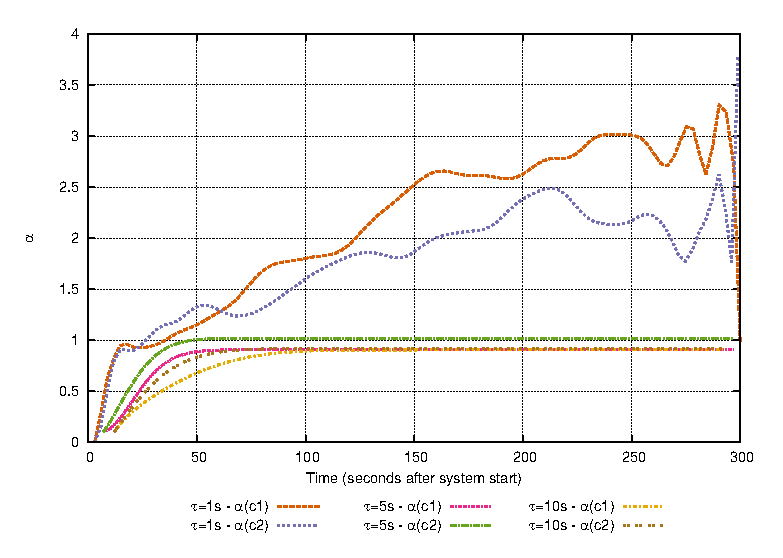
\includegraphics[scale=0.6]{figs/alpha.eps}  
\end{center}
% \vspace{-20pt}
\caption{{\scriptsize Evolving $\alpha(s,\tau,t_c)$ with different $\tau$}}
\label{fig:alpha}
% \vspace{-20pt}
% \end{wrapfigure}
\end{figure}
%

Every monitoring measurement is performed in a monitoring window $\tau$.
Monitoring measurements are aggregated and calculated in every window and form the basis of reactions necessary to evolve the service to meet their SLA.
Thus, selection of an appropriate monitoring window length $\tau$ is crucial, as we also discussed how schedulability analysis can be used to optimize it.
The authors in \cite{hogben2013defavail} present that for the same setup and deployment of services, measurements using different monitoring windows yield to very different understanding of service properties such as service availability.
Therefore, it is essential to choose the value of $\tau$ such that monitoring measurements do not lead to \emph{unrealistic} understanding and inappropriate reactions.

If $\tau < t_i$, Theorem \ref{thm:alpha} does not hold because every task \jtt{allocate} in $M_{\jtt{A}}$ misses its deadline.
Thus, it is essential that $\tau \geq t_i$.
Analogously, choosing monitoring window as $\tau \gg 2 \times t_i$ also has a counter-productive effect on the service deployments.
% 
% Assumption \ref{def:single:resource:type} says all the resources are of the same type and as such $t_i$ is the same for all resources.
In a real setting, different services may use different types of resources.
In such a setting, the monitoring window should be chosen as the largest $t_i$ of any resource type that is available in the platform: $\tau \geq \mathsf{max}(t_i) \; \forall r \in P$.

% section implementation (end)

